\PassOptionsToPackage{dvipsnames}{xcolor}
\documentclass[11pt,aspectratio=169]{beamer}
% metadata
\def\github{github.com/jessexknight/latex}
\title[\LaTeX: A Short Introduction]{\LaTeX\\\textsc{\small{A Short Introduction}}}
\author[\href{\github}{\tiny\texttt{\github}} \hspace{0.3\linewidth} Jesse Knight]
{Jesse Knight}
\institute{University of Toronto\\Libraries}
\date{2020 January 16}
\usepackage{graphicx,tikz,array}
\usepackage{bm,amsmath}
\usepackage{hyperref,xpatch,listings}
\usepackage[export]{adjustbox}
\usepackage[backend=biber,style=numeric,maxcitenames=1,sorting=none,
            isbn=false,url=true,doi=false,eprint=false]{biblatex}
% package configuration
\graphicspath{{figs/}}
\bibliography{../loi/refs.bib}
\lstset{
  language=[LaTeX]TeX,
  breaklines=true,
  basicstyle=\tt\scriptsize,
  texcsstyle=*\color{C2},
  identifierstyle=\color[HTML]{999999},
  commentstyle=\color{C3},
}
% styling
% beamer style
\usetheme{Malmoe}
\definecolor{C1}{HTML}{00204E}
\definecolor{C2}{HTML}{0099D2}
\definecolor{C3}{HTML}{BB133E}
\setbeamercolor{title}     {fg=C1}
\setbeamercolor{frametitle}{fg=C1}
\setbeamercolor{structure} {fg=C1}
\setbeamercolor{label}     {fg=C2}
\setbeamercolor{section}   {fg=white,bg=C1}
\setbeamercolor{subsection}{fg=white,bg=C1!60!white}
\setbeamercolor{link}      {fg=white,bg=C1}
\setbeamersize{text margin left=2em,text margin right=2em}
\setbeamertemplate{frametitle continuation}{}
\setbeamertemplate{bibliography item}{\colortext{C2}{\insertbiblabel}}
\setbeamertemplate{caption}{\centering\footnotesize{\insertcaption}\par}
\usefonttheme{serif}
\beamertemplatetransparentcoveredhigh
% colors
\let\oldcite=\cite
\renewcommand{\cite}[1]{\textcolor{purple}{\oldcite{#1}}}
% misc
\renewcommand*{\bibfont}{\tiny}
\setlength{\parskip}{0pt}
\setlength{\tabcolsep}{6pt}
\setlength{\belowcaptionskip}{-8pt}
% footer & frame number
\newcommand{\hfilll}{
  \hfill\hfill\hfill\hfill\hfill\hfill\hfill\hfill}
\expandafter\def\expandafter\insertshorttitle\expandafter{%
  \insertshorttitle\hfilll%
  \insertframenumber\,/\,\inserttotalframenumber}
\let\oldshortauthor=\insertshortauthor
\renewcommand{\insertshortauthor}{\textcolor{gray}{\oldshortauthor}}
\beamertemplatenavigationsymbolsempty
\setbeamercolor{itemize item}{fg=C1!100!white}
\setbeamercolor{itemize subitem}{fg=C1!60!white}
\setlength{\leftmargini}{6pt}
\settowidth{\leftmargini}{\usebeamertemplate{itemize item}}
\addtolength{\leftmargini}{\labelsep}
\xpatchcmd{\itemize}{\def\makelabel}{\setlength{\itemsep}{0.7em}\def\makelabel}{}{}
% itemize spacing
\let\tmpitemize\itemize
\let\tmpenditemize\enditemize
\renewenvironment{itemize}{\tmpitemize\addtolength{\itemsep}{-0.1\baselineskip}}{\tmpenditemize}
% tex commands
\newcommand{\colortext}[2]{{\color{#1}{#2}}}
\renewcommand{\ss}[1]{\textsuperscript{#1}}
\newcommand{\arrow}[1]{\hspace{#1}\colortext{C2}{$\bm\rightarrow$}\hspace{#1}}
\newcommand{\hreftt}[1]{\href{#1}{\colortext{C2}{\footnotesize\texttt{#1}}}}
\newcommand{\hrefc}[2]{\href{#1}{\colortext{C2}{#2}}}
\usetikzlibrary{arrows.meta}
\newcommand{\bigarrow}[2][C3]{%
  \begin{tikzpicture}
  \draw[->,>=Latex,line width=1mm,rounded corners,draw=#1](0,0)--(#2);
  \end{tikzpicture}
}

%%%%%%%%%%%%%%%%%%%%%%%%%%%%%%%%%%%%%%%%%%%%%%%%%%%%%%%%%%%%%%%%%%%%%%%%%%%%%%%%%%%%%%%%%%%%%%%%%%%%
\begin{document}
%%%%%%%%%%%%%%%%%%%%%%%%%%%%%%%%%%%%%%%%%%%%%%%%%%%%%%%%%%%%%%%%%%%%%%%%%%%%%%%%%%%%%%%%%%%%%%%%%%%%
\begin{frame}
  \maketitle
\end{frame}
%---------------------------------------------------------------------------------------------------
\begin{frame}[label=overview]{Overview}
  \tableofcontents
\end{frame}
%%%%%%%%%%%%%%%%%%%%%%%%%%%%%%%%%%%%%%%%%%%%%%%%%%%%%%%%%%%%%%%%%%%%%%%%%%%%%%%%%%%%%%%%%%%%%%%%%%%%
\section{Introduction}
%---------------------------------------------------------------------------------------------------
\begin{frame}{What is \LaTeX?}
  \pause
  A typesetting program:
  \pause
  \textit{content} $\rightarrow$ \textit{a document}
\end{frame}
%---------------------------------------------------------------------------------------------------
\begin{frame}{}
  \centering
  \begin{tabular}{m{0.4\linewidth} m{1cm} m{0.4\linewidth}}
    \parbox{\linewidth}{\centering input: \texttt{filename.tex}}
    & \LaTeX &
    \parbox{\linewidth}{\centering output: \texttt{filename.pdf}}
    \\[0.5em]
    \frame{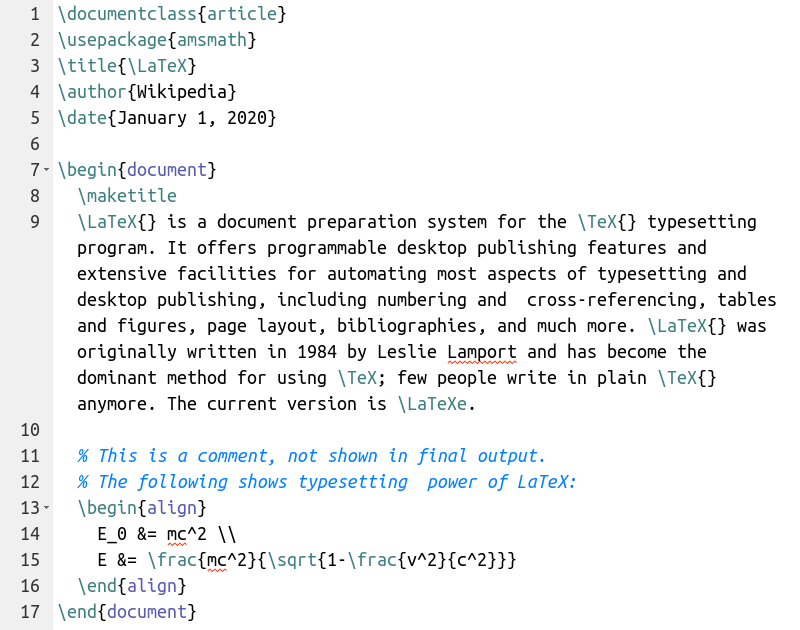
\includegraphics[width=\linewidth]{io-in.png}}
    & \bigarrow{1,0} &
    \frame{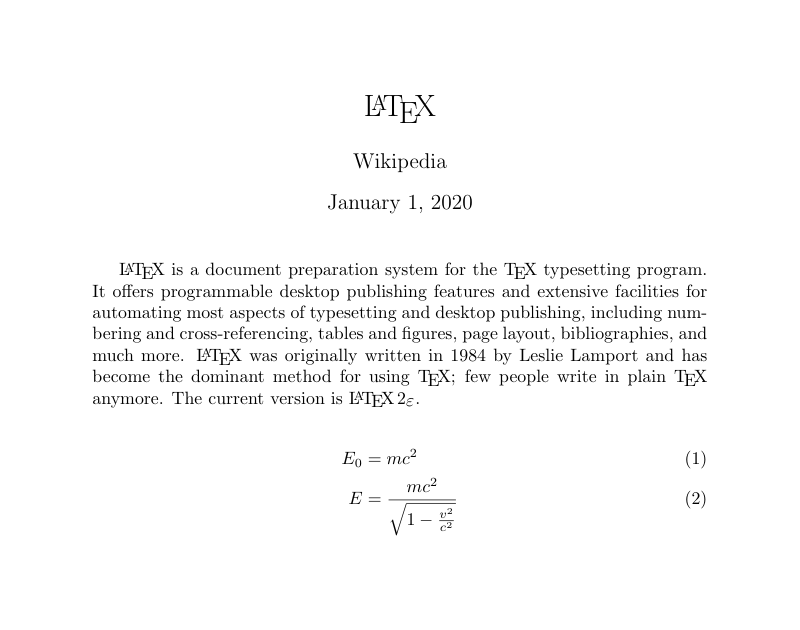
\includegraphics[width=\linewidth]{io-out.png}}
  \end{tabular}
\end{frame}
%---------------------------------------------------------------------------------------------------
\begin{frame}{Advantages of \LaTeX}
  \pause
  \begin{itemize}
    \item<+-> separate content and formatting
    \item<+-> automate numbering, cross-references, \dots everything!
    \item<+-> beautiful math
    \item<+-> comments and version control
    \item<+-> no version compatibility issues
    \item<+-> it's free!
  \end{itemize}
\end{frame}
%---------------------------------------------------------------------------------------------------
\begin{frame}{\LaTeX\ vs MS Word}
  \begin{figure}
    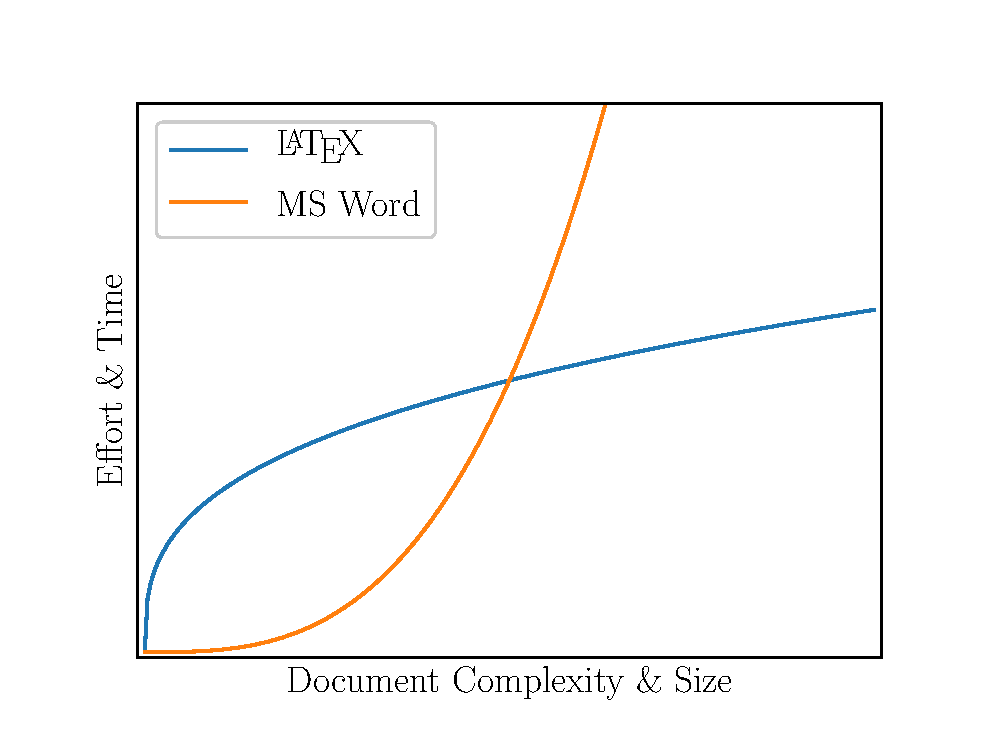
\includegraphics[width=0.6\linewidth]{latex-vs-word}
  \end{figure}
\end{frame}
%---------------------------------------------------------------------------------------------------
\begin{frame}[fragile]{How does \LaTeX\ Work?}
  Three layers:
  \begin{enumerate}
    \pause\item\parbox{2.3cm}{``primitives''} -- e.g.\ \lstinline|\def\pi{3.14}| defines a macro \lstinline|\pi| to contain ``3.14''\\[0.2em]
         \pause\parbox{2.3cm}{+ ``kernel''}   -- e.g.\ tools to combine primitives
    \pause\item\parbox{2.3cm}{``classes''}    -- e.g.\ an article, which should have: title, author, sections, etc.\\[0.2em]
         \pause\parbox{2.3cm}{+ ``packages''} -- e.g.\ modify or extend a basic class
    \pause\item\parbox{2.3cm}{``document''}   -- e.g.\ this specific article (including content!)
  \end{enumerate}
\end{frame}
%%%%%%%%%%%%%%%%%%%%%%%%%%%%%%%%%%%%%%%%%%%%%%%%%%%%%%%%%%%%%%%%%%%%%%%%%%%%%%%%%%%%%%%%%%%%%%%%%%%%
\section{Getting Started}
%---------------------------------------------------------------------------------------------------
\begin{frame}[fragile]{Your First Document}
  \begin{minipage}{0.44\linewidth}
    \begin{lstlisting}
\documentclass{article}
% document header
\begin{document}
  % document content
  Hello World
\end{document}
    \end{lstlisting}
  \end{minipage}
  \pause
  \begin{minipage}{0.55\linewidth}
    But first: \hrefc{https://www.overleaf.com}{Overleaf}
    \pause
    $\rightarrow$ ``New Project''
  \end{minipage}
\end{frame}
%---------------------------------------------------------------------------------------------------
\begin{frame}{Document Elements}
  \pause
  \begin{itemize}
    \item<+-> title, author, date
    \item<+-> sections
    \item<+-> math
    \item<+-> floats: figures \& tables
    \item<+-> cross-references \& table of contents
    \item<+-> citations \& bibliography
    \item<+-> appendices \& code
  \end{itemize}
\end{frame}
%%%%%%%%%%%%%%%%%%%%%%%%%%%%%%%%%%%%%%%%%%%%%%%%%%%%%%%%%%%%%%%%%%%%%%%%%%%%%%%%%%%%%%%%%%%%%%%%%%%%
\section{Examples}
%---------------------------------------------------------------------------------------------------
\begin{frame}{Putting it all Together}
  \pause
  \begin{itemize}
    \item<+-> \parbox{2cm}{e.g.\ thesis:}  \footnotesize\texttt{examples/thesis/main.pdf}
    \item<+-> \parbox{2cm}{e.g.\ CV:}      \footnotesize\texttt{examples/cv/main.pdf}
    \item<+-> \parbox{2cm}{e.g.\ article:} \footnotesize\texttt{examples/article/main.pdf}
    \item<+-> \parbox{2cm}{e.g.\ article:} \footnotesize\texttt{examples/poster/main.pdf}
  \end{itemize}
\end{frame}
%---------------------------------------------------------------------------------------------------
\begin{frame}[fragile]{Helpful Resources}
\newcommand{\linkbox}[2]{\parbox{3.5cm}{\hrefc{#1}{#2}}}
  \begin{itemize}
    \item \linkbox{https://www.overleaf.com}{Overleaf}
    -- online \LaTeX\ writing application\\
    \item \linkbox{https://www.latex-tutorial.com/installation}{\LaTeX\ Install Guide}
    -- to install \LaTeX\ on your computer (offline)\\
    \item \linkbox{https://www.texstudio.org}{TeXstudio}
    -- great editor for composing \LaTeX\ ``code'' (offline)\\
    \item \linkbox{https://tex.stackexchange.com}{\TeX\ Stack Exchange}
    -- Q \& A style how-to and debugging help
    \item \linkbox{https://wch.github.io/latexsheet/latexsheet.pdf}{\LaTeX\ Cheat Sheet}
    -- a really nice reference for common commands
    \item \linkbox{https://github.com/jessexknight/latex}{Github Repository}
    -- example documents: article, thesis, CV, poster, slides
  \end{itemize}
\end{frame}
%%%%%%%%%%%%%%%%%%%%%%%%%%%%%%%%%%%%%%%%%%%%%%%%%%%%%%%%%%%%%%%%%%%%%%%%%%%%%%%%%%%%%%%%%%%%%%%%%%%%
\end{document}
%%%%%%%%%%%%%%%%%%%%%%%%%%%%%%%%%%%%%%%%%%%%%%%%%%%%%%%%%%%%%%%%%%%%%%%%%%%%%%%%%%%%%%%%%%%%%%%%%%%%